\documentclass[20pt]{report}
\usepackage{amsmath, amssymb,amsmath}

\usepackage[spanish, es-lcroman]{babel}  
\usepackage[spanish]{babel}
\usepackage{multicol}
\usepackage{graphicx}
\usepackage{makeidx}
\usepackage{multicol}
 \cleardoublepage
\usepackage{graphicx}
\usepackage{float}
\providecommand{\abs}[1]{\lvert#1\rvert}
\providecommand{\norm}[1]{\lVert#1\rVert}
\usepackage{listings}
\usepackage{fancybox}
\usepackage{cancel}
%\usepackage{float}
\usepackage{wrapfig}
\parindent=2.1pc
\setlength{\oddsidemargin}{0.5cm} \setlength{\evensidemargin}{0cm}
\setlength{\textwidth}{16cm} \setlength{\textheight}{23cm}
\setlength{\topmargin}{-.5cm}
\begin{document}

\begin{figure}[H]
  \scalebox{0.5}{
    
\includegraphics[scale=1]{1.jpg} 
    %\caption{Descripci\'on si se desea} 
    }
\end{figure}

\begin{figure}[H]
  \scalebox{0.5}{
  
    
\includegraphics[scale=0.5]{udec4.jpg} 
    %\caption{Descripci\'on si se desea} 
    }
    \centering
\end{figure}


\topmargin=-1.6cm

%%%%%%%%%%%%%%%%%%%%% ENCABEZADO %%%%%%%%%%%%%%%%%%%%%%%%%%%%%%%%

\vspace{1cm}

\noindent\rule{15cm}{.5pt}

\begin{center}
\noindent{\huge\textbf{{UNIVERSIDAD DE CONCEPCI\'ON}}}\\
\noindent{\Large\textbf{{FACULTAD DE CIENCIAS F\'ISICAS Y MATEM\'ATICAS }}}\\

{DEPARTAMENTO DE INGENIER\'IA EN MATEM\'ATICA}
\end{center}
\begin{center}
\noindent\rule{15cm}{.5pt}\\
\vspace{2cm}
\textbf{\Large{ CARTOGRAMA	 DE CHILE}}\\

\Large{Sebasti\'an Moraga Scheuermann}\\

\Large{Profesor Dr. Leonardo Figueroa}\\

\end{center}
%\vspace{0.5cm} \centerline{\bf \large } 



 %\centerline{\bf \large Ingenier\'ia Civil Matem\'atica}\\
 %\centerline{\bf \large Universidad de Concepci\'on}
%%%%%%%%%%%%%%%%%%%%%%%%%%%%%%%%%%%%%%%%%%%%%%%%%%%%%%%%%%%%%%%%%
 \vspace{.2cm}
  \noindent
%%%%%%%%%%%%%%%%%%%%%%%%%%%%%%%%%%%%%%%%%%%%%%%%%%%%%%%%%%%%%%%%%
\begin{itemize}
\item [\bf ]{\bf    }
\topmargin=-1.6cm


\end{itemize}
\topmargin=-1.6cm
\vspace{3cm}
\noindent 



%\rule{16cm}{.5pt} 



\pagebreak


 \tableofcontents % indice de contenidos


\chapter{Introducci\'on}\label{cap.introduccion}

\pagenumbering{arabic} % para empezar la numeraci\'on con n\'umeros
Un cartograma es un mapa que muestra gr\'aficamente datos de un lugar geogr\'afico alterando su  imagen,  por medio de alg\'un patr\'on o medida de \'area que sea identificable  y f\'acilmente interpretable.\\
 El siguiente texto trata sobre  la creaci\'on de un cartograma de Chile basado en el m\'etodo de difusi\'on de Gastner/Newman [2004], que adapta mapas seg\'un la densidad de una regi\'on sin alterar sus relaciones  con otras regiones.
 \\
 \\
A medida que ha pasado el tiempo se han creado varios m\'etodos de c\'omo crear un cartograma,  pero todos de ellos con alg\'un problema como fuerte dependencia de los ejes coordenados que se usan, o simplemente problemas al tener zonas que se sobreponen, esto entre otros problemas.
\\
\\
    
Un archivo .shp  es un archivo con informaci\'on sobre alguna regi\'on,  l\'imites, adem\'as de contener las delimitaciones de las zonas puede almacenar  distintas variables como poblaci\'on, densidad,  o cualquier otro atributo que se le quiera asignar a alguna zona. Este es el archivo con el cual  trabajaremos para crear el cartograma, adem\'as fue usado el programa QGIS 2.18.1 para agregar atributos a un archivo division\_comunal.shp y as\'i poder trabajar con \'el. 
\pagebreak



\chapter{Enunciado }\label{cap.introduccion}
\section{ Inter\'es}
\begin{itemize}
\item Sea $\Omega$ la superficie de la Rep\'ublica de Chile y sea $\rho$ una aproximaci\'on de la funci\'on densidad-humana definida sobre $\Omega$. Queremos tener un cartograma de Chile a partir de la informaci\'on regida del censo 2012
\\
\begin{figure}[H]
\begin{center}
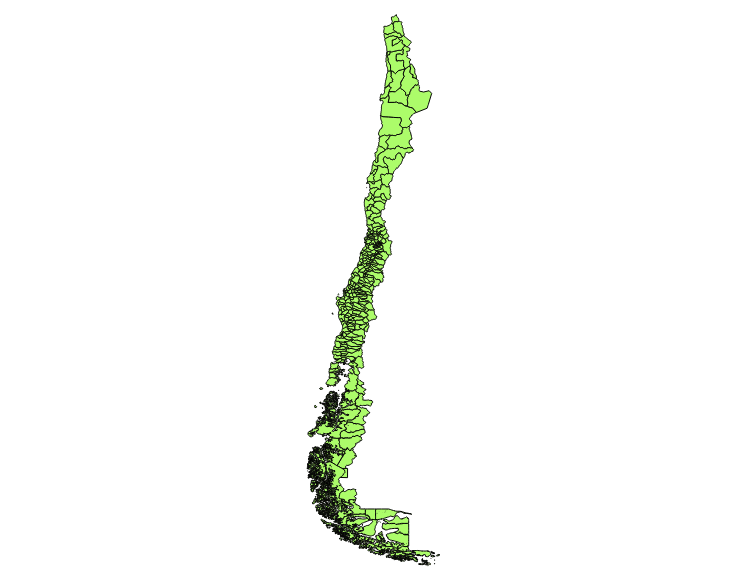
\includegraphics[width=10cm, height=10cm]{Chile.png}
\vspace{-0.5cm} %Espacio vertical negativo para pegar mas el caption de la figura a la propia figura
\caption{Chile continental}
\label{Label para referencia}
\end{center}
\end{figure}



\pagebreak
\label{cap.introduccion}\section{Base te\'orica}

Este proyecto es una aplicaci\'on del trabajo realizado en el paper "Diffusion-based method for producing
density-equalizing maps'' creado por   "Michael T. Gastner and M. E. J. Newman''  es claro que su m\'etodo ser\'a explicado en lo que sigue y se mostrar\'an los resultados obtenidos. \\\\

B\'asicamente se  realiza es describir la poblaci\'on  por una funci\'on densidad $\rho (r)$ donde $r$ es la posici\'on geogr\'afica, y de ello vamos a obtener la difusi\'on. Tal como se describe en el paper, a medida que $t\longrightarrow \infty$  la densidad completa del mapa geogr\'afico se vuelve  uniforme y el desplazamiento total determina la proyecci\'on necesaria para obtener el cartograma.
El procedimiento completo est\'a explicado en su paper, sin embargo resaltaremos lo m\'as importante,  que es la construcci\'on de la soluci\'on y  los m\'etodos usados.
\\
En difusi\'on estandar la densidad actual est\'a dada por
\begin{equation}
J= v(r,t)\rho (r,t)
\end{equation}
Donde $v(r,t)$ y $\rho(r,t)$ son la velocidad y la densidad respectivamente, con $r$ y $t$ la posici\'on y el tiempo. Adem\'as el gradiente del campo densidad es

\begin{equation}
J=-\nabla \rho
\end{equation}
lo que indica que el flujo  va en direcci\'on  de  m\'as densidad a donde hay menos, se indica que podemos omitir  una constante de difusi\'on  que podr\'ia aparecer en la ecuaci\'on anterior, asumirla como $1$. Entonces la difusi\'on de poblaci\'on es conservada localmente  as\'i que  se tiene 
\begin{equation}
\nabla \cdot J + \dfrac{\partial \rho}{\partial t} =0
\end{equation}
Combinando estas ecuaciones se tiene la ecucaci\'on de difusi\'on:
\begin{equation}
\nabla ^2 \rho - \dfrac{\partial \rho }{\partial t}=0
\end{equation}
y la expresi\'onde del  campo velocidad en t\'erminos de la densidad de poblaci\'on es:
\begin{equation}
v(r,t)= - \dfrac{\nabla \rho}{\rho}
\end{equation}


Para calcular el cartograma  se debe resolver la ecuaci\'on (2.4) para $\rho(r,t)$. Bajo las condiciones  mencionadas en el paper se tiene que se resolvi\'o la ecuaci\'on de difusi\'on en  espacios de Fourier,  el cual es diagonal y se vuelve a la transoformada antes de integrar sobre el campo de velocidades, con esto y  con las condiciones de borde del tipo  Newmann, la base de Fourier  de cosenos  en cuyo caso la soluci\'on a la ecuaci\'on de difusi\'on tienen la forma
\begin{equation}
\rho (r,t)= \dfrac{4}{L_x L_y} \sum_k {\overline{\rho}} (k) \cos(k_x x) \cos(k_y y)exp(-k^2 t)
\end{equation}
Tales que $L_x,L_y$ son las dimensiones de la zona rectangular  donde se encontrar\'a el mapa, en el cual son  lo suficientemente m\'as amplias que las propias coordenadas de las regiones para efectos de la difusi\'on. \\
La suma est\'a calculada sobre los vectores $k=(k_x,k_y)=2 \pi (m/L_x, n/L_y)$ con m, n enteros no negativos y $\overline{\rho}(k$ es la transformacion discreta del coseno de $\rho (r, t=0)$:
\begin{equation}
\overline{\rho}(k)=\dfrac{1}{4}(\delta_{k_x,0}+1)(\delta_{k_y,0}+1)\times \int_0^{L_x} \int_0^{L_y} \rho (r,0)\cos(k_x x)\cos(k_y y) dx dy
\end{equation}


\pagebreak
Donde $\delta_{i,j}$ es el delta de Kronecker. El campo de velocidades $v$ es facilmente calculable de la ecuaci\'on (2.5) y (2.6)  y tiene componentes
\begin{equation}
v_x(r,t)=\dfrac{\sum_k {k_x\overline{\rho}} (k) \sin(k_x x) \cos(k_y y)exp(-k^2 t)}{\sum_k {\overline{\rho}} (k) \cos(k_x x) \cos(k_y y)exp(-k^2 t)}
\end{equation}
\begin{equation}
v_y(r,t)=\dfrac{\sum_k {k_y\overline{\rho}} (k) \cos(k_x x) \sin(k_y y)exp(-k^2 t)}{\sum_k {\overline{\rho}} (k) \cos(k_x x) \cos(k_y y)exp(-k^2 t)}
\end{equation}
Ecuaciones (2.7), (2.8), (2.9) pueden ser r\'apidamente evaluadas usando la r\'apida transformada de Fourier (FFT) y su inversa respectivamente,  cada una  en un tiempo del orden $L_x L_y log(L_x L_y)$. Entonces se usa  el campo de velocidades restante para integrar la ecuaci\'on 
\[r(t)= r(0) +\int_0^t v(r,\tau)d\tau\]
Que es el desplazamiento acumulativo de cualquier punto del mapa al tiempo $t$.
\\
Esto genera una ecuaci\'on  Volterra no lineal de segundo tipo que puede ser resuelta num\'ericamente por m\'etodos est\'andar.



Esta es la base te\'orica en la que se bas\'o el proyecto del cartograma para Chile, as\'i pues  el software ScapeToad  creado por Dominique Andrieu, Christian Kaiser y Andr\'e Ourednik  hace uso  del dise\~no para crear cartogramas de Michael T. Gastner and M. E. J. Newman, el cual se alimenta de un archivo .shp  que contiene los datos, la forma  y de limitaciones de regiones que  queremos cartografiar, adem\'as de la densidad de cada regi\'on. Es por ello que ocupando el programa "QGIS Las" se retiraron zonas de chile que no eran pr\'oximas a Chile continental, tales como Isla de Pascua o Juan Fern\'andes pues al estar alejadas no producen distorsi\'on en lo que es  Chile continental. \\\\

Luego el archivo original division\_comunal.shp tampoco contaba con la densidad de cada regi\'on, por lo que se debi\'o  manualmente  crear ese campo de valores y establecerlos de acuerdo al censo sacado de Wikipedia. \\
As\'i  se fue completando este archivo arduamente hasta obtener todo lo necesario, luego simplemente se dej\'o correr el programa ScapeToad creando una matriz de $334 \times 2000$  sobre la imagen de Chile, al cual a cada nodo con  coordenadas $(x,y)$ se le asigna un valor de densidad, el cual   hace uso de la t\'ecnica antes descrita.
\pagebreak

\label{cap.introduccion}\section{Resultados num\'ericos} 
En la secci\'on siguiente tenemos los resultados de los cartogramas de Chile.\\
El programa funcion\'o durante  83719 segundos, o lo que es $23.2552$ horas continuas. \\
Esto llevo a los siguentes resultados \\\\

\item Error medio: $67.64444810600732$\\
\item Valor m\'aximo de densidad: $14218.14$.\\
\item Valor m\'inimo de densidad: $0.0$\\
\item Valor medio=$844.8950872093021$\\
\item N\'umero de comunas: $344$\\
\item Iteraciones: $3$\\
\item Diffusion grid size: $1024$\\
\item Cartogram grid size: $334 \times 2000$\\



\pagebreak

\begin{figure}[H]
\begin{center}
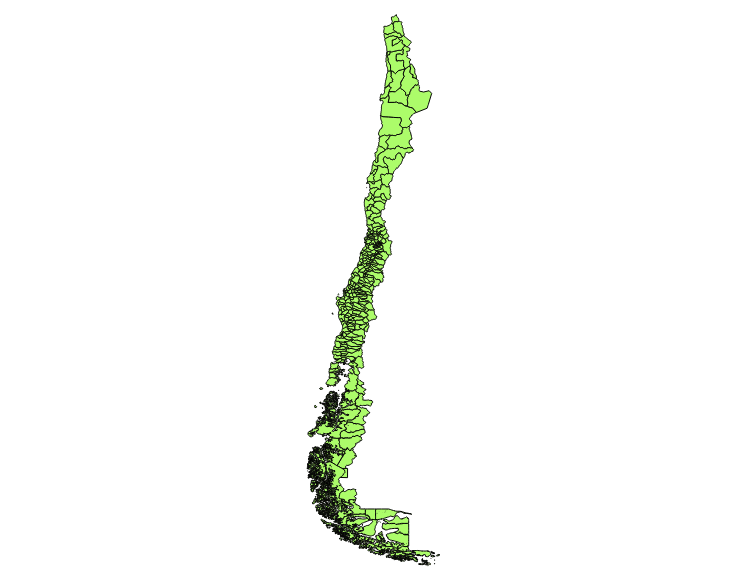
\includegraphics[width=10cm, height=10cm]{Chile.png}
\vspace{-0.5cm} %Espacio vertical negativo para pegar mas el caption de la figura a la propia figura
\caption{Chile continental sin difusi\'on}
\label{Label para referencia}
\end{center}
\end{figure}
\begin{figure}[H]
\begin{center}
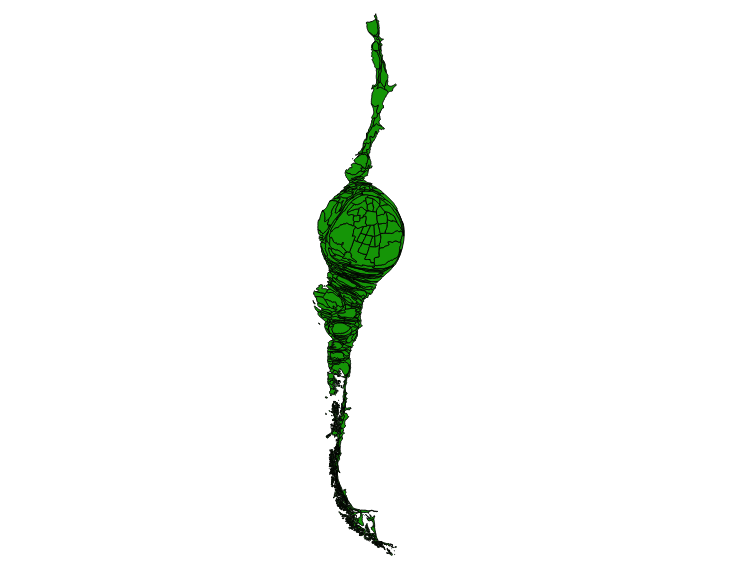
\includegraphics[width=10cm, height=10cm]{cartograma.png}
\vspace{-0.5cm} %Espacio vertical negativo para pegar mas el caption de la figura a la propia figura
\caption{Chile continental con difusi\'on}
\label{Label para referencia}
\end{center}
\end{figure}
Lo siguiente es la grilla sobre la cual se hicieron los c\'alculos, es visible que hicieron falta bastantes puntos para poder tener una buena aproximaci\'on. El tiempo de ejecuci\'on fue de $23.25$ horas, es claro que con menos iteraciones y una  con menos puntos puede tardar solo minutos pero la calidad del cartograma se pierde enormemente.
\begin{figure}[H]
\begin{center}
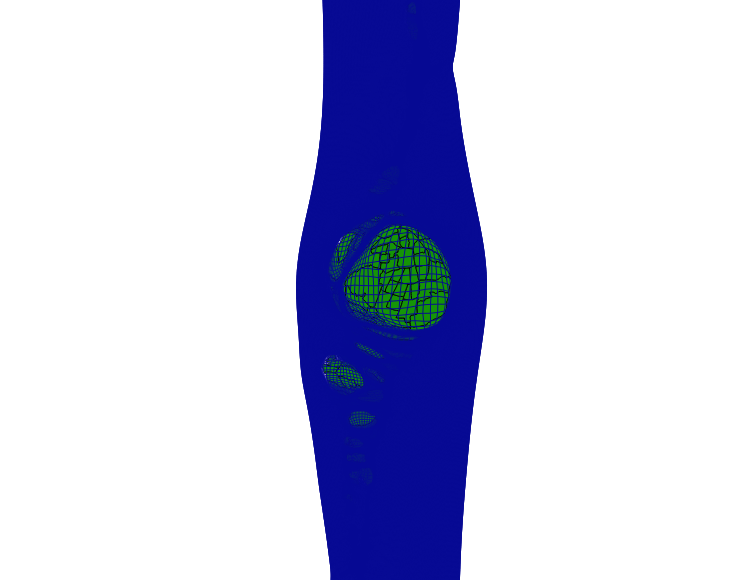
\includegraphics[width=5cm, height=5cm]{grilla.png}
\vspace{-0.5cm} %Espacio vertical negativo para pegar mas el caption de la figura a la propia figura
\caption{grilla sobre Chile}
\label{Label para referencia}
\end{center}
\end{figure}
\begin{figure}[H]
\begin{center}
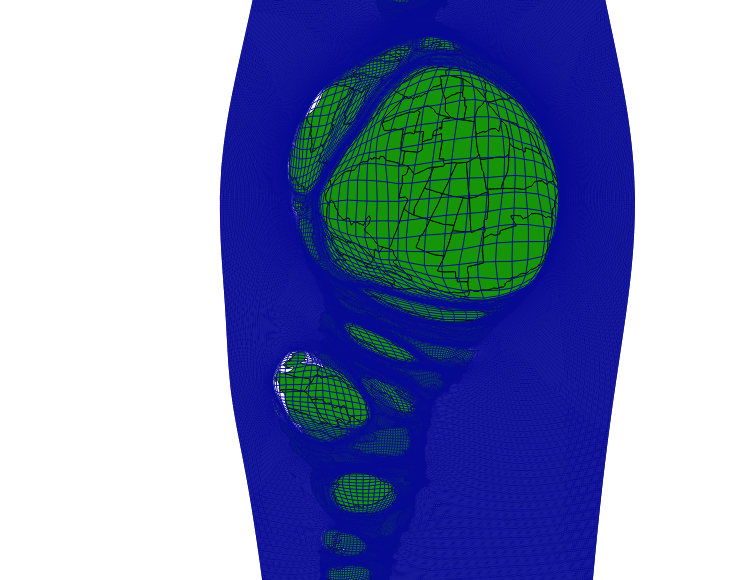
\includegraphics[width=10cm, height=10cm]{grillacentro.png}
\vspace{-0.5cm} %Espacio vertical negativo para pegar mas el caption de la figura a la propia figura
\caption{grilla sobre centro de Chile}
\label{Label para referencia}
\end{center}
\end{figure}
\pagebreak
Luego comenzamos a recorrer algunas comunas  de Chile, algunas importantes o destacadas.\\
Arica en el norte de Chile se muestra en la figura 2.6. Notando as\'i que su las zonas aleda\~nas contienen poblaci\'on mucho menor que esta comuna. Est\'a en el lugar $131$ de la lista de densidades, ordenada de mayor a menor.
\begin{figure}[H]
\begin{center}
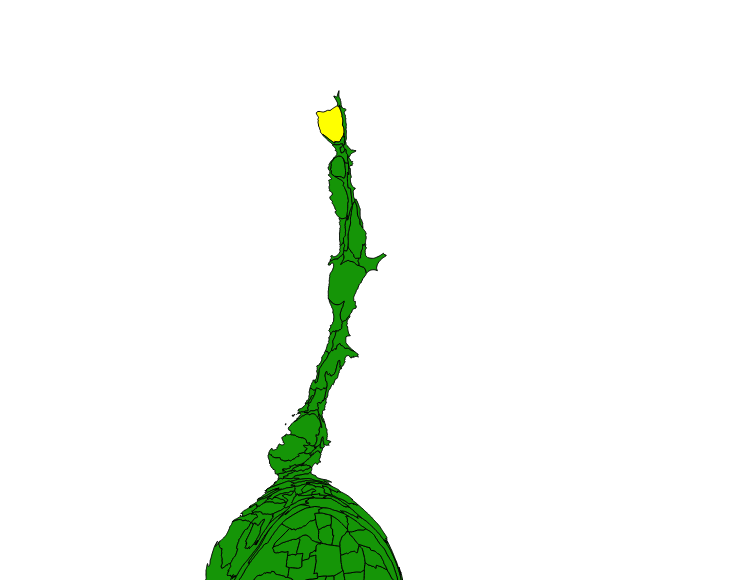
\includegraphics[width=8cm, height=8cm]{arica133.png}
\vspace{-0.5cm} %Espacio vertical negativo para pegar mas el caption de la figura a la propia figura
\caption{Norte de Chile: Arica}
\label{Label para referencia}
\end{center}
\end{figure}
La siguiente es la comuna de Putaendo que est\'a en el lugar $245$ de comunas, con una densidad aproximada de $10,41 Hab/km^2$.


\begin{figure}[H]
\begin{center}
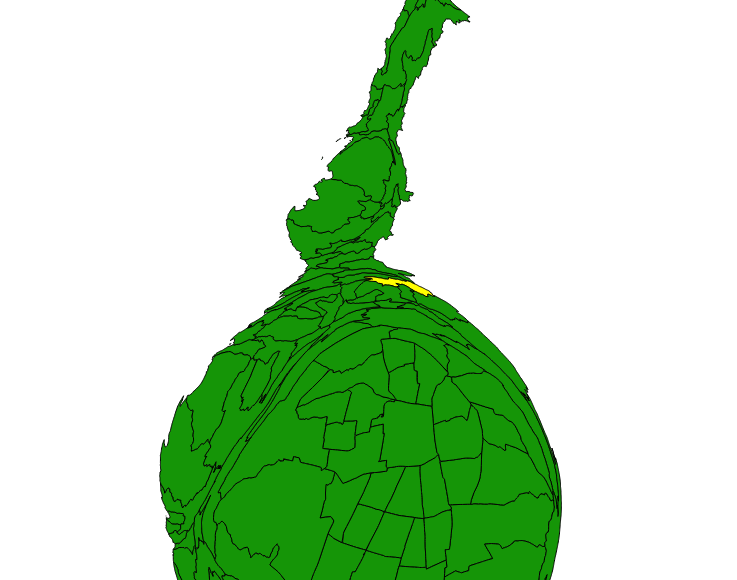
\includegraphics[width=8cm, height=8cm]{putaendo.png}
\vspace{-0.5cm} %Espacio vertical negativo para pegar mas el caption de la figura a la propia figura
\caption{Centro de Chile: Putaendo}
\label{Label para referencia}
\end{center}
\end{figure}
\pagebreak

La siguiente comuna es Lo espejo de la regi\'on metropolitana, la cual es la comuna con mayor densidad poblacional en Chile con alrededor de $14.218 Hab/km^2$. Aunque su densidad es mucho m\'as grande que Putaendo, Lo espejo no se deforma tan dr\'asticamente  debido a las otras comunas alrededor que tienen una densidad  parecida.
\begin{figure}[H]
\begin{center}
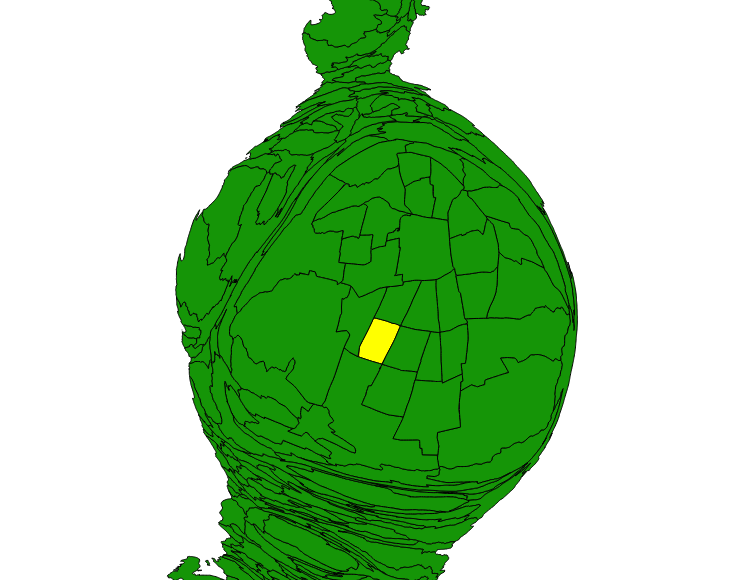
\includegraphics[width=10cm, height=10cm]{loespejo.png}
\vspace{-0.5cm} %Espacio vertical negativo para pegar mas el caption de la figura a la propia figura
\caption{Centro de Chile: Comuna de Lo espejo}
\label{Label para referencia}
\end{center}
\end{figure}
\pagebreak

En lo que sigue se presentar\'an comunas de Norte a Sur con su lugar en la lista de densidades.

\begin{figure}[H]
\begin{center}
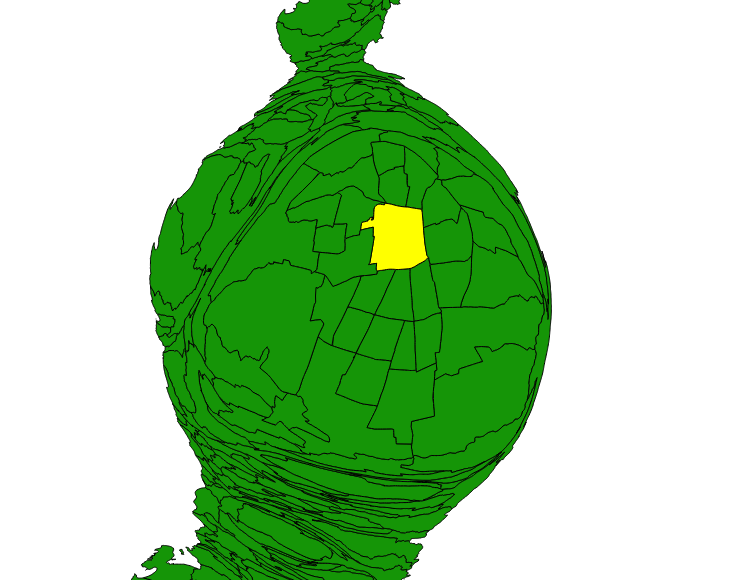
\includegraphics[width=10cm, height=10cm]{santiago9.png}
\vspace{-0.5cm} %Espacio vertical negativo para pegar mas el caption de la figura a la propia figura
\caption{Centro de Chile: Santiago, puesto $9^{no}$}
\label{Label para referencia}
\end{center}
\end{figure}

\begin{figure}[H]
\begin{center}
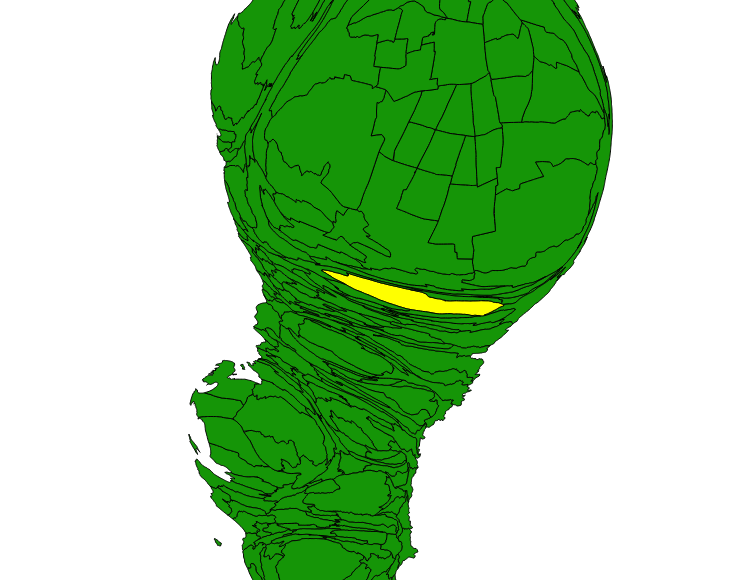
\includegraphics[width=10cm, height=10cm]{rancagua.png}
\vspace{-0.5cm} %Espacio vertical negativo para pegar mas el caption de la figura a la propia figura
\caption{Centro de Chile: Rancagua, puesto $41$}
\label{Label para referencia}
\end{center}
\end{figure}

\begin{figure}[H]
\begin{center}
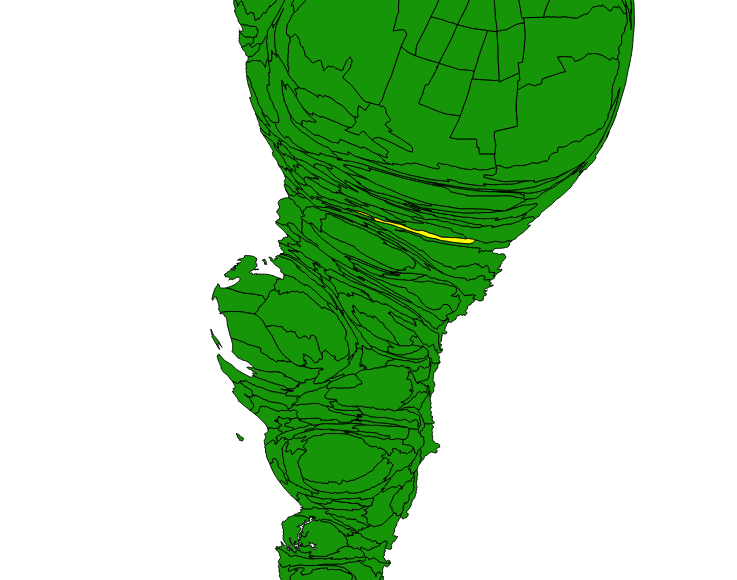
\includegraphics[width=5cm, height=5cm]{teno129.png}
\vspace{-0.5cm} %Espacio vertical negativo para pegar mas el caption de la figura a la propia figura
\caption{Centro de Chile: Teno, puesto $127$}
\label{Label para referencia}
\end{center}
\end{figure}

\begin{figure}[H]
\begin{center}
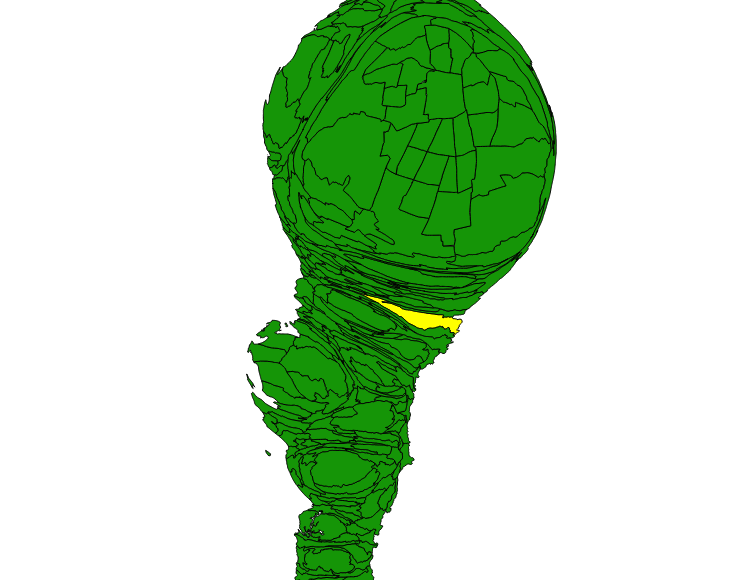
\includegraphics[width=10cm, height=10cm]{curico79.png}
\vspace{-0.5cm} %Espacio vertical negativo para pegar mas el caption de la figura a la propia figura
\caption{Centro de Chile: Curic\'o, puesto $77$}
\label{Label para referencia}
\end{center}
\end{figure}



\begin{figure}[H]
\begin{center}
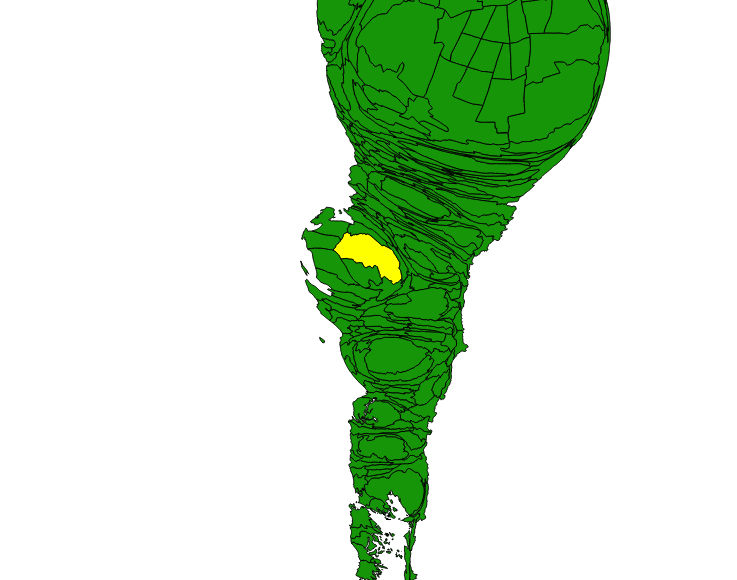
\includegraphics[width=10cm, height=10cm]{concepcion42.png}
\vspace{-0.5cm} %Espacio vertical negativo para pegar mas el caption de la figura a la propia figura
\caption{Centro de Chile: Concepci\'on, puesto $36$}
\label{Label para referencia}
\end{center}
\end{figure}





\begin{figure}[H]
\begin{center}
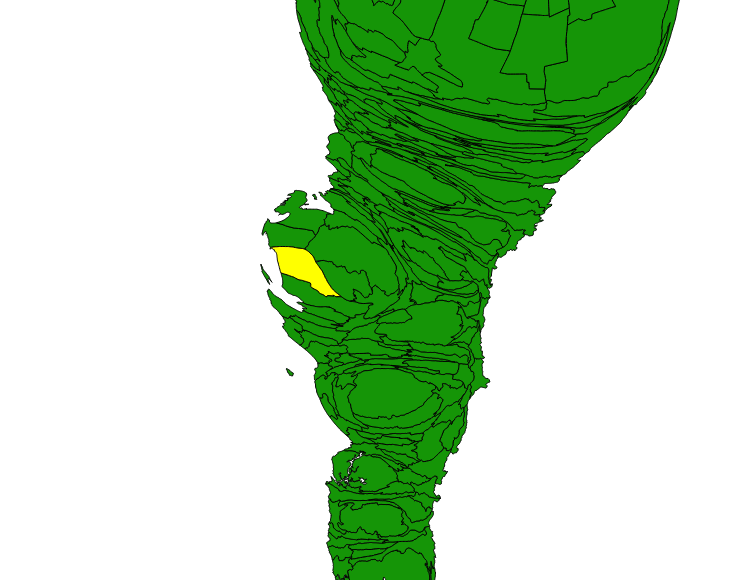
\includegraphics[width=10cm, height=10cm]{sanpedro.png}
\vspace{-0.5cm} %Espacio vertical negativo para pegar mas el caption de la figura a la propia figura
\caption{Centro de Chile: San Pedro de la Paz, puesto $43$}
\label{Label para referencia}
\end{center}
\end{figure}

\begin{figure}[H]
\begin{center}
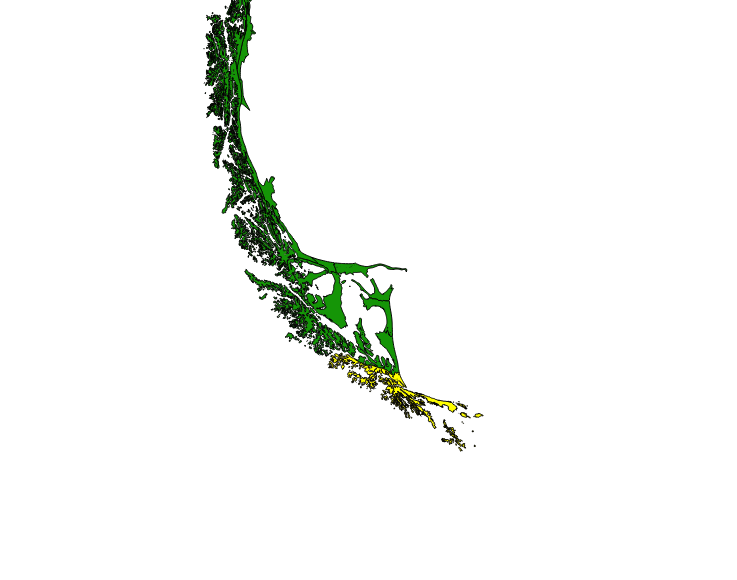
\includegraphics[width=10cm, height=10cm]{cabodehornos.png}
\vspace{-0.5cm} %Espacio vertical negativo para pegar mas el caption de la figura a la propia figura
\caption{Sur de Chile: Cabo de Hornos, puesto $335$}
\label{Label para referencia}
\end{center}
\end{figure}










\begin{figure}[H]
\begin{center}
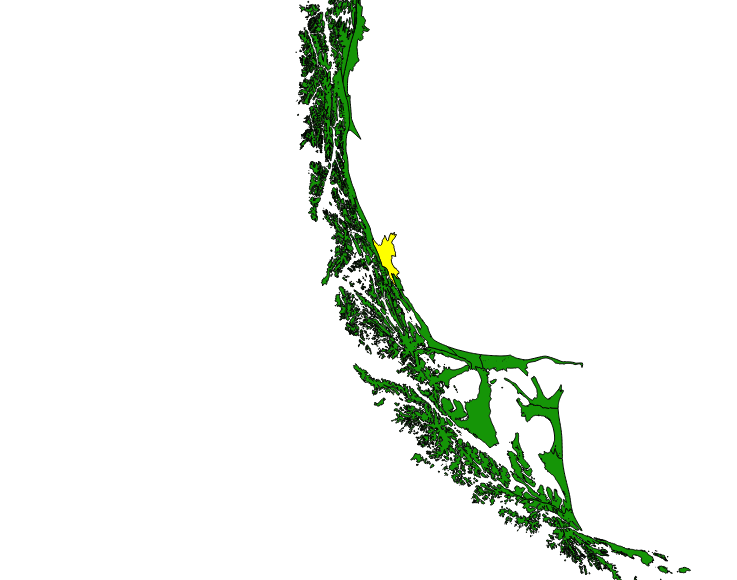
\includegraphics[width=10cm, height=10cm]{torresdelpaine340.png}
\vspace{-0.5cm} %Espacio vertical negativo para pegar mas el caption de la figura a la propia figura
\caption{Sur de Chile: Torres del Paine, puesto $340$}
\label{Label para referencia}
\end{center}
\end{figure}
\section{Conclusiones}
El proyecto est\'a basado en una s\'olida base te\'orica, la cual se puso en pr\'actica para saber cu\'al ser\'ia el cartograma de Chile deformado seg\'un la densidad poblacional de \'este mismo. Es claro que aun se conserva la imagen visual de un Chile alargado, sin embargo se hace presente la concentraci\'on de gente en la capital del pa\'is  y zona centro,  lo cual en cifras era conocido, pero ahora tenemos un ejemplo visual que lo apoya.\\
 Aunque el mapeo tiene un cierto error asociado  es una buena reprecentaci\'on; si se quisiera un cartograma con mayor detalle es posible, sin embargo, el tiempo  de ejecuci\'on se reflejar\'ia en  varios d\'ias dependiendo de la r\'apidez del  computador. Para efectos visuales el cartograma presentado en este informe es aceptable.
 \\
 \\
 
 Para trabajo futuro, ser\'ia interesante lograr a nivel de  algunas pocas comunas  un mayor detalle logrando as\'i deformar  aspectos reconocibles de  una regi\'on, tales como r\'ios, lagos, carreteras, etc. No se realiz\'o  en este informe por cuesti\'on de tiempo, ya que se requiere de un manejo pleno en el programa editor Qgis. 
\section{Recomendaciones}
Se adjunta un archivo llamado cartograma.shp que contiene el cartograma de Chile por si  el lector desea revisarla, esto es posible mediante el programa QGIS $2.18.1$ de licencia gratuita. Adem\'as incluido va un archivo Deformation grid.shp el cual tiene la grilla  con la que se realiz\'o el cartograma de Chile. \\
El lector podr\'a realizar su propio cartograma con ScapeToad-v11 que tambi\'en est\'a incluido. Se recomienda  hacer un cartograma de baja calidad  debido al tiempo de ejecuci\'on.
\pagebreak

\section{Bibliografia}
\item http://  www.bcn.cl /textbackslash siit/mapas\_ vectoriales/ index\_ html
\item https://es.wikipedia.org/wiki/Anexo:Comunas\_de\_Chile
\item Gastner, M.T. and Newman, M. (2004). Diffusion-based method for producing density equalizing maps. In Proceedings of the National Academy of Sciences of the United States of America, 101(20): 7499-7504.
\item http://scapetoad.choros.ch/index.php
\item Qgis Software, Lic. GNU,http://www.qgis.org/
\end{itemize}
\end{document}

